\section{Einführung}

\begin{takeaway}
    \item NP-schwer vs. NP-vollständig
    \item Schwellwertsprache
\end{takeaway}

\paragraph{Polynomzeit-Reduzierbarkeit}
Ein Entscheidungsproblem $\Pi_1$ ist ``polynomzeit-reduzierbar'' auf ein anderes
Entscheidungsproblem $\Pi_2$:
\begin{align*}
& \Longleftrightarrow
\exists \text{ Algo } \A \text{ s.t. } \Time_\A \in \text{poly}
\wedge \Pi_1(x) = \Pi_2(\A(x))
\\
& \Longleftrightarrow
\Pi_2 \text{ mindestens so schwer wie } \Pi_1
\\
& \Longleftrightarrow
\Pi_1 \text{ höchstens so schwer wie } \Pi_2
\\
& \Longleftrightarrow
\Pi_1 \preceq_P \Pi_2
\end{align*}

\paragraph{NP-schwer (NP-hard)}
Ein Problem $\Pi$ das ``mindestens so schwer'' ist wie alle Probleme in NP.
D.h. alle Probleme in NP lassen sich auf $\Pi$ reduzieren:
$$ \forall \Pi' \in NP : \Pi' \preceq_P \Pi $$
$\Pi$ muss nicht notwendigerweise in NP liegen (d.h. kann schwerer sein)!
Beispiel: das Halteproblem (nicht entscheidbar, daher $\notin NP$).

\paragraph{NP-vollständig (NP-complete)}
Ein Problem $\Pi$, das in NP liegt \underline{und} NP-schwer ist.
``Repräsentativ'' für die Menge NP, da sich alle Probleme aus NP darauf reduzieren lassen. \\
Beispiel: Satisfiability-Problem SAT (Satz von Cook).

\begin{figure}[h]
    \centering
	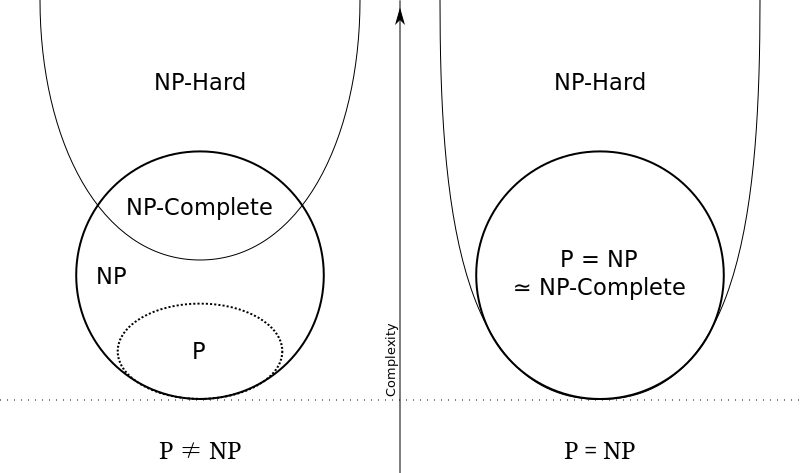
\includegraphics[scale=0.4]{images/np-hard-complete.png}
    \caption{Mengendiagramm der Beziehungen (Quelle: \href{https://commons.wikimedia.org/w/index.php?curid=3532181}{Wikipedia})}
    \label{fig:pke-ind-cca}
\end{figure}

\paragraph{``Schwere Probleme''}
NP-schwere Probleme, aber generell alle Probleme die sich nicht in Polynomzeit lösen lassen.
\textbf{Sinnvollerweise gehen wir im Folgenden davon aus dass $P \neq NP$.}

Alle Instanzen unseres Problems sind deterministisch in Polynomzeit \underline{nicht} lösbar.
Mögliche Ansätze:
\begin{enumerate}[label=\alph*)]
    \item nicht exakt sondern approximativ lösen (Approximationsalgorithmen)
    \item nicht deterministisch sondern nichtdeterministisch lösen (Randomisierte Algorithmen)
    \item nicht polynomiell sondern moderat exponentiell lösen%
    \footnote{D.h. die Basis der Exponentation ist klein, z.B. $1.4^n$ statt $2^n$.}
    \item nicht alle sondern alle Instanzen mit einer bestimmten Struktur lösen (Parametrisierte Algorithmen)
    \item anderweitig zusätzliche Informationen über die Eingabe nutzen (Reoptimierung, Win-Win-Strategy)
    \item Heuristiken\footnote{Nachteil: Im Gegensatz zu den anderen Ansätzen ist hier die Qualität (Laufzeit, ...) nicht beweisbar.}
\end{enumerate}


\subsection{Definitionen}

\paragraph{Entscheidungsproblem}
$P = (L, U, \Sigma)$ wobei
\begin{itemize}
    \item $\Sigma$ ein Alphabet
    \item $U \subseteq \Sigma^*$ die Menge der zulässigen Eingaben (als Wörter über dem Alphabet, als \emph{Sprache})
    \item $L \subseteq U$ die Menge der akzeptierten Eingaben (\emph{JA-Instanzen})
\end{itemize}
Ein Algorithmus $\A$ \emph{löst} $P$ falls gilt:
$$ \forall u \in U : A(x) =
\begin{cases}
1 \text{ oder JA}, \text{ if } x \in L \\
0 \text{ oder NEIN}, \text{ if } x \in U-L \\
\end{cases}
$$

\paragraph{Vertex Cover Problem VC}
``Der Hefepilz der parametrisierten Algorithmiker -- ein Modellproblem.''
\\
Eingabe $U$: ungerichteter Graph $G = (V, E)$ und $k \leq |V|, k \in \N$. \\
Ausgabe $L$: JA falls $\exists C \subseteq V$ s.t. $|C| \leq k$ mit $\forall \{u, v \} \in E: u \in C \vee v \in V$.

\paragraph{Satisfiability-Problem SAT} \mbox{} \\
Eingabe: CNF-Formel $\Phi = C_1 \wedge \dots \wedge C_m$ mit Klauseln $C_i$ über Variablen $x_1, \dots, x_n$. \\
Ausgabe: eine Variablen-Belegung die $\Phi$ erfüllt.

Bei $l$-SAT enthält jede Klausel maximal $l$ Literale.

\paragraph{Optimierungsproblem}
$U = (L, M, cost, goal)$ wobei
\begin{itemize}
    \item $L$ die Sprache der zulässigen Eingaben\footnote{Oben noch $U$!}
    \item $\M: L \mapsto \Sigma^*$ so dass $M(x)$ die Sprache der akzeptierten Lösungen für Eingabe $x$
    \item $cost$: $\forall x \in L \; \forall y \in M(x) : cost(y, x) = $ Kosten der Lösung $y$ für Eingabe $x$
    \item $goal \in \{ \min, \max \}$ das Optimierungsziel
    \item $Opt_U(x) = goal \{ cost(y, x) | y \in M(x) \}$ die Kosten einer optimalen Lösung für Eingabe $x$
\end{itemize}

\paragraph{Minimum Vertex Cover Problem MIN-VC}
Wie VC, mit $cost(C, G) = |C| = $ Grösse des Vertex Covers und $goal = \min$.

\paragraph{MAX-SAT}
Wie SAT, mit $cost = $ Anzahl belegte Variablen und $goal = \max$.

\paragraph{Laufzeit}
eines Algorithmus' $\A$ auf Eingabe $x$ ist $\Time_\A (x)$
wobei $\Time_\A: \N \mapsto \N$.
Die Laufzeit von $\A$ in Abhängigkeit von der Grösse $n$ der Eingabe ist:
$\Time_\A (n) = \max \{ \Time_\A (x) \; | \; |x| = n, x \in L \}$.
Die Laufzeit wird in  $\bigO$-Notation angegeben.

\paragraph{Schwellwertsprache (threshold language)} definiert für ein Optimierungsproblem $U$:
$$ Lang_U = \{ (x, a) \in L \times \binarystring \; | \; Opt_U(x) \leq Number(a) \} $$
wo $Number(a)$ die Zahl mit der Binärdarstellung $a$ (der \emph{Schwellwert}) ist und $goal = \min$.
\\
Beispiel: $Lang_{MIN-VC} = VC$. Aber $Lang_{MAX-SAT} \neq SAT$ (da SAT leichter sein kann)!

$U$ heisst ``NP-schwer'' falls $Lang_U$ NP-schwer ist (warum?).%
\footnote{Recall that NP-Schwere für Entscheidungsprobleme definiert ist.
Über die Schwellwertsprache erweitern wir dies für Optimierungsprobleme.}
